\mysection{Plus loin avec les pointeurs}
\myindex{\CLanguageElements!\Pointers}
\label{label_pointers}

\epigraph{The way C handles pointers, for example, was a brilliant innovation;
it solved a lot of problems that we had before in data structuring and
made the programs look good afterwards.}{Donald Knuth, interview (1993)}

Pour ceux qui veulent se casser la tête à comprendre les pointeurs \CCpp, voici plus
d'exemples.
Certains d'entre eux sont bizarres et ne servent qu'à des fins de démonstration:
utilisez-les en production uniquement si vous savez vraiment ce que vous faites.

\subsection{Travailler avec des adresses au lieu de pointeurs}

Un pointeur est juste une adresse en mémoire. Mais pourquoi écrivons-nous \TT{char* string}
au lieu de quelque chose comme \TT{address string}?
La variable pointeur est fournie avec un type de la valeur sur laquelle le pointeur
pointe.
Donc le compilateur est capable de détecter des bugs de type de données lors de la
compilation.

Pour être pédant, les types de données des langages de programmation ne servent qu'a
prévenir des bugs et à l'auto-documentation.
Il est possible de n'utiliser que deux types de données, comme \IT{int} (ou \IT{int64\_t})
et l'octet---ce sont les seuls types disponible aux programmeurs en langage d'assemblage.
Mais c'est une tâche extrêmement difficile d'écrire des programmes en assembleur
pratique et sans bugs méchants.
La plus petite typo peut conduire à un bug difficile-à-trouver.

L'information sur le type de données est absente d'un code compilé (et c'est l'un
des problèmes majeurs pour les dé-compilateurs), et je peux le prouver.

Ceci est ce qu'un programmeur \CCpp peut écrire:

\begin{lstlisting}[style=customc]
#include <stdio.h>
#include <stdint.h>

void print_string (char *s)
{
	printf ("(address: 0x%llx)\n", s);
	printf ("%s\n", s);
};

int main()
{
	char *s="Hello, world!";

	print_string (s);
};
\end{lstlisting}

Ceci est ce que je peux écrire:

\begin{lstlisting}[style=customc]
#include <stdio.h>
#include <stdint.h>

void print_string (uint64_t address)
{
	printf ("(address: 0x%llx)\n", address);
	puts ((char*)address);
};

int main()
{
	char *s="Hello, world!";

	print_string ((uint64_t)s);
};
\end{lstlisting}

J'utilise \IT{uint64\_t} car j'ai effectué cet exemple sur Linux x64. \IT{int} fonctionnerait
pour des \ac{OS}-s 32-bit.
D'abord, un pointeur sur un caractère (la toute première chaîne de bienvenu) est
casté en \IT{uint64\_t}, puis passé plus loin.
La fonction \TT{print\_string()} re-caste la valeur \IT{uint64\_t} en un pointeur
sur un caractère.

Ce qui est intéressant, c'est que GCC 4.8.4 produit une sortie assembleur identique
pour les deux versions:

\begin{lstlisting}
gcc 1.c -S -masm=intel -O3 -fno-inline
\end{lstlisting}

\begin{lstlisting}[style=customasmx86]
.LC0:
	.string	"(address: 0x%llx)\n"
print_string:
	push	rbx
	mov	rdx, rdi
	mov	rbx, rdi
	mov	esi, OFFSET FLAT:.LC0
	mov	edi, 1
	xor	eax, eax
	call	__printf_chk
	mov	rdi, rbx
	pop	rbx
	jmp	puts
.LC1:
	.string	"Hello, world!"
main:
	sub	rsp, 8
	mov	edi, OFFSET FLAT:.LC1
	call	print_string
	add	rsp, 8
	ret
\end{lstlisting}

(j'ai supprimé toutes les directives non significatives de GCC.)

J'ai aussi essayé différents utilitaires UNIX de \IT{diff} et ils ne montrent aucune
différence.

Continuons à abuser massivement des traditions de programmation de \CCpp.
On pourrait écrire ceci:

\begin{lstlisting}[style=customc]
#include <stdio.h>
#include <stdint.h>

uint8_t load_byte_at_address (uint8_t* address)
{
	return *address;
	//this is also possible: return address[0]; 
};

void print_string (char *s)
{
	char* current_address=s;
	while (1)
	{
		char current_char=load_byte_at_address(current_address);
		if (current_char==0)
			break;
		printf ("%c", current_char);
		current_address++;
	};
};

int main()
{
	char *s="Hello, world!";

	print_string (s);
};
\end{lstlisting}

Ça pourrait être récrit comme ceci:

\begin{lstlisting}[style=customc]
#include <stdio.h>
#include <stdint.h>

uint8_t load_byte_at_address (uint64_t address)
{
	return *(uint8_t*)address;
};

void print_string (uint64_t address)
{
	uint64_t current_address=address;
	while (1)
	{
		char current_char=load_byte_at_address(current_address);
		if (current_char==0)
			break;
		printf ("%c", current_char);
		current_address++;
	};
};

int main()
{
	char *s="Hello, world!";

	print_string ((uint64_t)s);
};
\end{lstlisting}

Les deux codes source donnent la même sortie assembleur:

\begin{lstlisting}
gcc 1.c -S -masm=intel -O3 -fno-inline
\end{lstlisting}

\begin{lstlisting}[style=customasmx86]
load_byte_at_address:
	movzx	eax, BYTE PTR [rdi]
	ret
print_string:
.LFB15:
	push	rbx
	mov	rbx, rdi
	jmp	.L4
.L7:
	movsx	edi, al
	add	rbx, 1
	call	putchar
.L4:
	mov	rdi, rbx
	call	load_byte_at_address
	test	al, al
	jne	.L7
	pop	rbx
	ret
.LC0:
	.string	"Hello, world!"
main:
	sub	rsp, 8
	mov	edi, OFFSET FLAT:.LC0
	call	print_string
	add	rsp, 8
	ret
\end{lstlisting}

(j'ai supprimé toutes les directives non significatives de GCC.)

Aucune différence: les pointeurs \CCpp sont essentiellement des adresses, mais fournies
avec une information sur le type, afin de prévenir des erreurs possible lors de la
compilation.

\subsection{Passer des valeurs en tant que pointeurs; tagged unions}

Voici un exemple montrant comment passer des valeurs dans des pointeurs:

\begin{lstlisting}[label=unsigned_multiply_C,style=customc]
#include <stdio.h>
#include <stdint.h>

uint64_t multiply1 (uint64_t a, uint64_t b)
{
	return a*b;
};

uint64_t* multiply2 (uint64_t *a, uint64_t *b)
{
	return (uint64_t*)((uint64_t)a*(uint64_t)b);
};

int main()
{
	printf ("%d\n", multiply1(123, 456));
	printf ("%d\n", (uint64_t)multiply2((uint64_t*)123, (uint64_t*)456));
};
\end{lstlisting}

Il fonctionne sans problème et GCC 4.8.4 compile les fonctions multiply1() et multiply2()
de manière identique!

\begin{lstlisting}[label=unsigned_multiply_lst,style=customasmx86]
multiply1:
	mov	rax, rdi
	imul	rax, rsi
	ret

multiply2:
	mov	rax, rdi
	imul	rax, rsi
	ret
\end{lstlisting}

Tant que vous ne déréférencez pas le pointeur (autrement dit, que vous ne lisez aucune
donnée depuis l'adresse stockée dans le pointeur), tout se passera bien.
Un pointeur est une variable qui peut stocker n'importe quoi, comme une variable
usuelle.

\myindex{x86!\Instructions!MUL}
\myindex{x86!\Instructions!IMUL}
L'instruction de multiplication signée (\IMUL) est utilisée ici au lieu de la non-signée
(\MUL), lisez-en plus à ce sujet ici:
\ref{IMUL_over_MUL}.

\myindex{Tagged pointers}
À propos, il y a une astuce très connue pour abuser des pointeurs appelée \emph{tagged pointers}.
En gros, si tous vos pointeurs pointent sur des blocs de mémoire de taille, disons,
16 octets (ou qu'ils sont toujours alignés sur une limite de 16-octet), les 4 bits
les plus bas du pointeur sont toujours zéro et cet espace peut être utilisé d'une
certaine façon.
\myindex{LISP}
C'est très répandu dans les compilateurs et interpréteurs LISP.
Ils stockent le type de cell/objet dans ces bits inutilisés, ceci peut économiser
un peu de mémoire.
Encore mieux, vous pouvez évaluer le type de cell/objet en utilisant seulement le pointeur,
sans accès supplémentaire à la mémoire.
En lire plus à ce sujet: \InSqBrackets{\CNotes\ 1.3}.

% TODO Example of tagged ptrs here

\subsection{Abus de pointeurs dans le noyau Windows}

La section ressource d'un exécutable PE dans les OS Windows est une section contenant
des images, des icônes, des chaînes, etc.
Les premières versions de Windows permettaient seulement d'adresser les ressources
par ID, mais Microsoft a ajouté un moyen de les adresser en utilisant des chaînes.

Donc, il doit être alors possible de passer un ID ou une chaîne a la fonction
Elle est déclarée comme ceci:
\href{https://msdn.microsoft.com/en-us/library/windows/desktop/ms648042i\%28v=vs.85\%29.aspx}{FindResource()}.

\myindex{win32!FindResource()}

\begin{lstlisting}[style=customc]
HRSRC WINAPI FindResource(
  _In_opt_ HMODULE hModule,
  _In_     LPCTSTR lpName,
  _In_     LPCTSTR lpType
);
\end{lstlisting}

\IT{lpName} et \IT{lpType} ont un type \IT{char*} ou \IT{wchar*}, et lorsque quelqu'un 
veut encore passer un ID, il doit utiliser la macro
\href{https://msdn.microsoft.com/en-us/library/windows/desktop/ms648029\%28v=vs.85\%29.aspx}{MAKEINTRESOURCE},
comme ceci:

\myindex{win32!MAKEINTRESOURCE()}

\begin{lstlisting}[style=customc]
result = FindResource(..., MAKEINTRESOURCE(1234), ...);
\end{lstlisting}

C'est un fait intéressant que MAKEINTRESOURCE est juste un casting d'entier vers un pointeur.
Dans MSVC 2013, dans le fichier\\\IT{Microsoft SDKs\textbackslash{}Windows\textbackslash{}v7.1A\textbackslash{}Include\textbackslash{}Ks.h}
nous pouvons voir ceci:

\begin{lstlisting}[style=customc]
...

#if (!defined( MAKEINTRESOURCE )) 
#define MAKEINTRESOURCE( res ) ((ULONG_PTR) (USHORT) res)
#endif

...
\end{lstlisting}

Ça semble fou. Regardons dans l'ancien code source de Windows NT4 qui avait fuité.\\
Dans \IT{private/windows/base/client/module.c} nous pouvons trouver le source code
de \IT{FindResource()}:

\begin{lstlisting}[style=customc]
HRSRC
FindResourceA(
    HMODULE hModule,
    LPCSTR lpName,
    LPCSTR lpType
    )

...

{
    NTSTATUS Status;
    ULONG IdPath[ 3 ];
    PVOID p;

    IdPath[ 0 ] = 0;
    IdPath[ 1 ] = 0;
    try {
        if ((IdPath[ 0 ] = BaseDllMapResourceIdA( lpType )) == -1) {
            Status = STATUS_INVALID_PARAMETER;
            }
        else
        if ((IdPath[ 1 ] = BaseDllMapResourceIdA( lpName )) == -1) {
            Status = STATUS_INVALID_PARAMETER;
...
\end{lstlisting}

Continuons avec \IT{BaseDllMapResourceIdA()} dans le même fichier source:

\begin{lstlisting}[style=customc]
ULONG
BaseDllMapResourceIdA(
    LPCSTR lpId
    )
{
    NTSTATUS Status;
    ULONG Id;
    UNICODE_STRING UnicodeString;
    ANSI_STRING AnsiString;
    PWSTR s;

    try {
        if ((ULONG)lpId & LDR_RESOURCE_ID_NAME_MASK) {
            if (*lpId == '#') {
                Status = RtlCharToInteger( lpId+1, 10, &Id );
                if (!NT_SUCCESS( Status ) || Id & LDR_RESOURCE_ID_NAME_MASK) {
                    if (NT_SUCCESS( Status )) {
                        Status = STATUS_INVALID_PARAMETER;
                        }
                    BaseSetLastNTError( Status );
                    Id = (ULONG)-1;
                    }
                }
            else {
                RtlInitAnsiString( &AnsiString, lpId );
                Status = RtlAnsiStringToUnicodeString( &UnicodeString,
                                                       &AnsiString,
                                                       TRUE
                                                     );
                if (!NT_SUCCESS( Status )){
                    BaseSetLastNTError( Status );
                    Id = (ULONG)-1;
                    }
                else {
                    s = UnicodeString.Buffer;
                    while (*s != UNICODE_NULL) {
                        *s = RtlUpcaseUnicodeChar( *s );
                        s++;
                        }

                    Id = (ULONG)UnicodeString.Buffer;
                    }
                }
            }
        else {
            Id = (ULONG)lpId;
            }
        }
    except (EXCEPTION_EXECUTE_HANDLER) {
        BaseSetLastNTError( GetExceptionCode() );
        Id =  (ULONG)-1;
        }
    return Id;
}
\end{lstlisting}

\IT{lpId} est ANDé avec \IT{LDR\_RESOURCE\_ID\_NAME\_MASK}. Que nous pouvons trouver
dans \IT{public/sdk/inc/ntldr.h}:

\begin{lstlisting}[style=customc]
...

#define LDR_RESOURCE_ID_NAME_MASK 0xFFFF0000

...
\end{lstlisting}

Donc \IT{lpId} est ANDé avec \IT{0xFFFF0000} et si des bits sont encore présents
dans la partie 16-bit basse, la première partie de la fonction est exécutée (\IT{lpId} 
est traité comme une adresse de chaîne).
Autrement---la seconde moitié (\IT{lpId} est traitée comme une valeur 16-bit).

Encore, ce code peut être trouvé dans le fichier kernel32.dll de Windows 7:

\lstinputlisting[style=customasmx86]{advanced/450_more_ptrs/tmp1.lst}

Si la valeur du pointeur en entrée est plus grande que 0x10000, un saut au traitement
de chaînes se produit.
Autrement, la valeur en entrée du \IT{lpId} est renvoyée telle quelle.
Le masque \IT{0xFFFF0000} n'est plus utilisé ici, car ceci est du code 64-bit, mais
encore, \IT{0xFFFFFFFFFFFF0000} pourrait fonctionner ici.

Le lecteur attentif pourrait demander ce qui se passe si l'adresse de la chaîne en
entrée est plus petite que 0x10000?
Ce code se base sur le fait que dans Windows, il n'y a rien aux adresses en dessous
de 0x10000, au moins en Win32 realm.

Raymond Chen \href{https://blogs.msdn.microsoft.com/oldnewthing/20130925-00/?p=3123}{écrit} à propos de ceci:

\begin{framed}
\begin{quotation}
How does MAKE­INT­RESOURCE work? It just stashes the integer in the bottom 16 bits of a pointer, leaving the upper bits zero. This relies on the convention that the first 64KB of address space is never mapped to valid memory, a convention that is enforced starting in Windows 7.
\end{quotation}
\end{framed}

En quelques mots, ceci est un sale hack et probablement qu'il ne devrait être utilisé
qu'en cas de réelle nécessité.
Peut-être que la fonction \IT{FindResource()} avait un type \IT{SHORT} pour ses arguments,
et puis Microsoft a ajouté un moyen de passer des chaînes ici, mais que le code ancien
devait toujours être supporté.

Maintenant, voici un exemple distillé:

\begin{lstlisting}[style=customc]
#include <stdio.h>
#include <stdint.h>

void f(char* a)
{
	if (((uint64_t)a)>0x10000)
		printf ("Pointer to string has been passed: %s\n", a);
	else
		printf ("16-bit value has been passed: %d\n", (uint64_t)a);
};

int main()
{
	f("Hello!"); // pass string
	f((char*)1234); // pass 16-bit value
};
\end{lstlisting}

Ça fonctionne!

\subsubsection{Abus de pointeurs dans le noyau Linux}

Comme ça a déjà été pointé dans des \href{https://news.ycombinator.com/item?id=11823647}{commentaires sur Hacker News},
le noyau Linux comporte aussi des choses comme ça.

Par exemple, cette fonction peut renvoyer un code erreur ou un pointeur:

\begin{lstlisting}[style=customc]
struct kernfs_node *kernfs_create_link(struct kernfs_node *parent,
				       const char *name,
				       struct kernfs_node *target)
{
	struct kernfs_node *kn;
	int error;

	kn = kernfs_new_node(parent, name, S_IFLNK|S_IRWXUGO, KERNFS_LINK);
	if (!kn)
		return ERR_PTR(-ENOMEM);

	if (kernfs_ns_enabled(parent))
		kn->ns = target->ns;
	kn->symlink.target_kn = target;
	kernfs_get(target);	/* ref owned by symlink */

	error = kernfs_add_one(kn);
	if (!error)
		return kn;

	kernfs_put(kn);
	return ERR_PTR(error);
}
\end{lstlisting}

( \url{https://github.com/torvalds/linux/blob/fceef393a538134f03b778c5d2519e670269342f/fs/kernfs/symlink.c#L25} )

\IT{ERR\_PTR} est une macro pour caster un entier en un pointeur:

\begin{lstlisting}[style=customc]
static inline void * __must_check ERR_PTR(long error)
{
	return (void *) error;
}
\end{lstlisting}

( \url{https://github.com/torvalds/linux/blob/61d0b5a4b2777dcf5daef245e212b3c1fa8091ca/tools/virtio/linux/err.h} )

Ce fichier d'en-tête contient aussi une macro d'aide pour distinguer un code d'erreur
d'un pointeur:

\begin{lstlisting}[style=customc]
#define IS_ERR_VALUE(x) unlikely((x) >= (unsigned long)-MAX_ERRNO)
\end{lstlisting}

Ceci signifie que les codes erreurs sont les ``pointeurs'' qui sont très proche de
-1, et, heureusement, il n'y a rien dans la mémoire du noyau à des adresses comme
0xFFFFFFFFFFFFFFFF, 0xFFFFFFFFFFFFFFFE, 0xFFFFFFFFFFFFFFFD, etc.

Une méthode bien plus répandue est de renvoyer \IT{NULL} en cas d'erreur et de passer
le code d'erreur par un argument supplémentaire.
Les auteurs du noyau Linux ne font pas ça, mais quiconque veut utiliser ces fonctions
doit toujours garder en mémoire que le pointeur renvoyé doit toujours être testé avec
\IT{IS\_ERR\_VALUE} avant d'être déréférencé.

Par exemple:

\begin{lstlisting}[style=customc]
	fman->cam_offset = fman_muram_alloc(fman->muram, fman->cam_size);
	if (IS_ERR_VALUE(fman->cam_offset)) {
		dev_err(fman->dev, "%s: MURAM alloc for DMA CAM failed\n",
			__func__);
		return -ENOMEM;
	}
\end{lstlisting}

( \url{https://github.com/torvalds/linux/blob/aa00edc1287a693eadc7bc67a3d73555d969b35d/drivers/net/ethernet/freescale/fman/fman.c#L826} )

\subsubsection{Abus de pointeurs dans l'espace utilisateur UNIX}

\myindex{UNIX!mmap()}
La fonction mmap() renvoie -1 en cas d'erreur (ou \TT{MAP\_FAILED}, qui vaut -1).
Certaines personnes disent que mmap() peut mapper une zone mémoire à l'adresse zéro
dans de rares situations, donc elle ne peut pas utiliser 0 ou NULL comme code d'erreur.


\subsection{Pointeurs nuls}

\subsubsection{``Null pointer assignment'' erreur du temps de MS-DOS}

\myindex{MS-DOS}
Des anciens peuvent se souvenir d'un message d'erreur bizarre du temps de MS-DOS:
``Null pointer assignment''.
Qu'est-ce que ça signifie?

Il n'est pas possible d'écrire à l'adresse mémoire zéro avec les OSs *NIX et Windows,
mais il est possible de le faire avec MS-DOS, à cause de l'absence de protection
de la mémoire.

\myindex{Turbo C++}
\myindex{Borland C++}
Donc, j'ai sorti mon ancien Turbo C++ 3.0 (qui fût renommer plus tard en Borland C++)
d'avant les années 1990s et essayé de compiler ceci:

\begin{lstlisting}[style=customc]
#include <stdio.h>

int main()
{
	int *ptr=NULL;
	*ptr=1234;
	printf ("Now let's read at NULL\n");
	printf ("%d\n", *ptr);
};
\end{lstlisting}

C'est difficile à croire, mais ça fonctionne, sans erreur jusqu'à la sortie, toutefois:

\begin{lstlisting}[caption=Ancient Turbo C 3.0]
C:\TC30\BIN\1
Now let's read at NULL
1234
Null pointer assignment

C:\TC30\BIN>_
\end{lstlisting}

Plongeons un peu plus profondément dans le code du \ac{CRT} de Borland C++ 3.1, fichier \emph{c0.asm}:

\lstinputlisting[style=customasmx86]{advanced/450_more_ptrs/tmp2.lst}

Le modèle de mémoire de MS-DOS était vraiment bizarre (\ref{8086_memory_model}) et
ne vaut probablement pas la peine de s'y plonger, à moins d'être fan de rétro-computing
ou de rétro-gaming.
Une chose que nous devons garder à l'esprit est que le segment de mémoire (segment
de données inclus) dans MS-DOS, est un segment de mémoire dans lequel du code ou
des données sont stockés, mais contrairement au \ac{OS}s ``sérieux'', il commence
à l'adresse 0.

Et dans le \ac{CRT} de Borland C++, le segment de données commence avec 4 octets
à zéro puis la chaîne de copyright ``Borland C++ - Copyright 1991 Borland Intl.''.
L'intégrité des 4 octets à zéro et de la chaîne de texte est vérifiée en sortant,
et s'ils sont corrompus, le message d'erreur est affiché.

Mais pourquoi? Écrire à l'adresse zéro est une erreur courante en \CCpp, et si vous
faites cela sur *NIX ou Windows, votre application va planter.
MS-DOS n'a pas de protection de la mémoire, donc le \ac{CRT} doit vérifier ceci post-factum
et le signaler à la sortie.
Si vous voyez ce message, ceci signifie que votre programme à un certain point, a
écrit à l'adresse 0.

Notre programme le fait. Et ceci est pourquoi le nombre 1234 a été lu correctement:
car il a été écrit à la place des 4 premiers octets à zéro.
La somme de contrôle est incorrecte à la sortie (car le nombre y a été laissé), donc
le message a été affiché.

Ai-je raison?
J'ai récrit le programme pour vérifier mes suppositions:

\begin{lstlisting}[style=customc]
#include <stdio.h>

int main()
{
	int *ptr=NULL;
	*ptr=1234;
	printf ("Now let's read at NULL\n");
	printf ("%d\n", *ptr);
	*ptr=0; // psst, cover our tracks!
};
\end{lstlisting}

Ce programme s'exécute sans message d'erreur à la sortie.

Une telle méthode pour avertir en cas d'assignation du pointeur nul est pertinente
pour MS-DOS, peut-être qu'elle peut encore être utilisée de nos jours avec des \ac{MCU}s
à bas coût sans protection de la mémoire et/ou \ac{MMU}.

\subsubsection{Pourquoi voudrait-on écrire à l'adresse 0?}

Mais pourquoi un programmeur sain d'esprit écrirait du code écrivant quelque chose
à l'adresse 0?
Ça peut être fait accidentellement: par exemple, un pointeur doit être initialisé
au bloc de mémoire nouvellement alloué et ensuite passé à quelque fonction qui renvoie
des données à travers un pointeur.

\begin{lstlisting}[style=customc]
int *ptr=NULL;

\dots nous avons oublié d'allouer la mémoire et d'initialiser ptr

strcpy (ptr, buf); // strcpy() termine silencieusement car MS-DOS n'a pas de protection de la mémoire
\end{lstlisting}

Encore pire:

\begin{lstlisting}[style=customc]
int *ptr=malloc(1000);

\dots nous avons oublié de vérifier si la mémoire a réellement été allouée: c'est MS-DOS après tout et les ordinateurs ont une petite quantité de RAM,
\dots et être à court de RAM était très courant.
\dost si malloc() a renvoyé NULL, ptr sera aussi NULL.

strcpy (ptr, buf); // strcpy() termine silencieusement car MS-DOS n'a pas de protection de la mémoire
\end{lstlisting}

\subsubsection{NULL en \CCpp}

NULL en \CCpp est juste une macro qui est souvent définie comme ceci:

\begin{lstlisting}[style=customc]
#define NULL  ((void*)0)
\end{lstlisting}
( \href{https://github.com/wzhy90/linaro_toolchains/blob/8ff8ae680bac04558d10cc9626e12c4c2f6c1348/arm-cortex_a15-linux-gnueabihf/libc/usr/include/libio.h#L70}{fichier libio.h} )

\emph{void*} est un type de données reflétant le fait que c'est un pointeur, mais sur
une valeur d'un type de données inconnu (\emph{void}).

NULL est usuellement utilisé pour montrer l'absence d'un objet.
Par exemple, vous avez une liste simplement chaînée, et chaque n\oe{}ud a une valeur
(ou un pointeur sur une valeur) et un pointeur \emph{next}.
Pour montrer qu'il n'y a pas de n\oe{}ud suivant, 0 est stocké dans le champ \emph{next}.
(D'autres solutions sont pires.)
Peut-être pourriez-vous avoir un environnement fou où vous devriez allouer un bloc
de mémoire à l'adresse zéro. Comment indiqueriez-vous l'absence de n\oe{}ud suivant?
Avec une sorte de \emph{magic number}? Peut-être -1? Ou peut-être avec un bit additionnel?

Nous trouvons ceci dans Wikipédia:

\begin{framed}
\begin{quotation}
In fact, quite contrary to the zero page's original preferential use, some modern operating systems such as FreeBSD, Linux and Microsoft Windows[2] actually make the zero page inaccessible to trap uses of NULL pointers. 
\end{quotation}
\end{framed}
( \url{https://en.wikipedia.org/wiki/Zero_page} )

\subsubsection{Pointeur nul à une fonction}

Il est possible d'appeler une fonction avec son adresse.
Par exemple, je compile ceci avec MSVC 2010 et le lance dans Windows 7:

\begin{lstlisting}[style=customc]
#include <windows.h>
#include <stdio.h>

int main()
{
	printf ("0x%x\n", &MessageBoxA);
};
\end{lstlisting}

Le résultat est \emph{0x7578feae} et ne change pas après plusieurs lancements, car user32.dll
(où la fonction MessageBoxA se trouve) est toujours chargée à la même adresse.
Et aussi car \ac{ASLR} n'est pas activé (le résultat serait différent à chaque exécution
dans ce cas).

Appelons \emph{MessageBoxA()} par son adresse:

\begin{lstlisting}[style=customc]
#include <windows.h>
#include <stdio.h>

typedef int (*msgboxtype)(HWND hWnd, LPCTSTR lpText, LPCTSTR lpCaption,  UINT uType);

int main()
{
	msgboxtype msgboxaddr=0x7578feae;

	// force to load DLL into process memory, 
	// since our code doesn't use any function from user32.dll, 
	// and DLL is not imported
	LoadLibrary ("user32.dll");

	msgboxaddr(NULL, "Hello, world!", "hello", MB_OK);
};
\end{lstlisting}

Bizarre, mais ça fonctionne avec Windows 7 x86.

Ceci est communément utilisé dans les shellcodes, car il est difficile d'y appeler
des fonctions DLL par leur nom.
Et \ac{ASLR} est une contre-mesure.

Maintenant, ce qui est vraiment bizarre, quelques programmeurs C embarqué peuvent
être familiers avec un code comme ceci:

\begin{lstlisting}[style=customc]
int reset()
{
	void (*foo)(void) = 0;
	foo();
};
\end{lstlisting}

Qui voudrait appeler une fonction à l'adresse 0?
Ceci est un moyen portable de sauter à l'adresse zéro.
De nombreux micro-contrôleurs à bas coût n'ont pas de protection mémoire ou de \ac{MMU}
et après un reset, ils commencent à exécuter le code à l'adresse 0, où une sorte
de code d'initialisation est stocké.
Donc sauter à l'adresse 0 est un moyen de se réinitialiser.
On pourrait utiliser de l'assembleur inline, mais si ce n'est pas possible, cette
méthode portable est utilisable.

Ça compile même correctement avec mon GCC 4.8.4 sur Linux x64:

\begin{lstlisting}[style=customasmx86]
reset:
        sub     rsp, 8
        xor     eax, eax
        call    rax
        add     rsp, 8
        ret
\end{lstlisting}

Le fait que le pointeur de pile soit décalé n'est pas un problème: le code d'initialisation
dans les micro-contrôleurs ignorent en général les registres et l'état de la \ac{RAM}
et démarrent from scratch.

Et bien sûr, ce code planterait sur *NIX ou Windows à cause de la protection mémoire,
et même sans la protection mémoire, il n'y a pas de code à l'adresse 0.

GCC possède même des extensions non-standard, permettant de sauter à une adresse spécifique
plutôt qu'un appel à une fonction ici:
\url{http://gcc.gnu.org/onlinedocs/gcc/Labels-as-Values.html}.


\subsection{Tableaux comme argument de fonction}

On peut se demander quelle est la différence entre déclarer le type d'un argument
de fonction en tant que tableau et en tant que pointeur?

Il semble qu' il n'y ai pas du tout de différence:

\begin{lstlisting}[style=customc]
void write_something1(int a[16])
{
	a[5]=0;
};

void write_something2(int *a)
{
	a[5]=0;
};

int f()
{
	int a[16];
	write_something1(a);
	write_something2(a);
};
\end{lstlisting}

GCC 4.8.4 \Optimizing:

\begin{lstlisting}[style=customasmx86]
write_something1:
        mov     DWORD PTR [rdi+20], 0
        ret

write_something2:
        mov     DWORD PTR [rdi+20], 0
        ret
\end{lstlisting}

Mais vous pouvez toujours déclarer un tableau au lieu d'un pointeur à des fins d'auto-documentation,
si la taille du tableau est toujours fixée.
Et peut-être, des outils d'analyse statique seraient capable de vous avertir d'un
possible débordement de tampon.
Ou est-ce possible avec des outils aujourd'hui?

Certaines personnes, incluant Linux Torvalds, critiquent cette possibilité de \CCpp:
\url{https://lkml.org/lkml/2015/9/3/428}.

Le standard C99 a aussi le mot-clef \emph{static} \InSqBrackets{\CNineNineStd{} 6.7.5.3}:

\begin{framed}
\begin{quotation}
If the keyword static also appears  within the [ and ] of the array type derivation, then for each call to the function, the value of the corresponding actual argument shall provide access to the first element of an array with at least as many elements as specified by the size expression.
\end{quotation}
\end{framed}
Si le mot-clef static apparaît entre les [ et ] du tableau de dérivation de type, alors pour chaque appel à la fonction,


\subsection{Pointeur sur une fonction}

Un nom de fonction en \CCpp sans parenthèses, comme ``printf'' est un pointeur sur
une fonction du type \emph{void (*)()}.
Essayons de lire le contenu de la fonction et de la patcher:

\lstinputlisting[style=customc]{advanced/450_more_ptrs/6.c}

Ça dit que les 3 premiers octets de la fonction sont \TT{55 89 e5}.
En effet, ce sont les opcodes des instructions \INS{PUSH EBP} et \INS{MOV EBP, ESP}
(se sont des opcodes x86).
Mais alors notre programme plante, car la section \emph{text} est en lecture seule.

Nous pouvons recompiler notre exemple et rendre la section \emph{text} modifiable
\footnote{\url{http://stackoverflow.com/questions/27581279/make-text-segment-writable-elf}}:

\begin{lstlisting}
gcc --static -g -Wl,--omagic -o example example.c
\end{lstlisting}

Ça fonctionne!

\begin{lstlisting}
we are in print_something()
first 3 bytes: 55 89 e5...
going to call patched print_something():
it must exit at this point
\end{lstlisting}


\subsection{Pointeur comme un identificateur d'objet}

Tant le langage assembleur que le C n'ont pas de fonctionnalité \ac{OOP}, mais il
est possible d'écrire du code dans un style \ac{OOP} (il suffit de traiter une structure
comme un objet).

Il est intéressant que, parfois, un pointeur sur un objet (ou son adresse) soit appelé
comme ID (dans le sens de cacher/encapsuler des données).

\myindex{win32!LoadLibrary()}
\myindex{win32!GetProcAddress()}
Par exemple, LoadLibrary(), d'après \ac{MSDN}, renvoie une ``handle to the module''
\footnote{\url{https://msdn.microsoft.com/ru-ru/library/windows/desktop/ms684175(v=vs.85).aspx}}.
Puis, vous passez ce ``handle'' à une autre fonction comme GetProcAddress().
Mais en fait, LoadLibrary() renvoie un pointeur sur le fichier DLL mappé en mémoire.
\footnote{\url{https://blogs.msdn.microsoft.com/oldnewthing/20041025-00/?p=37483}}.
Vous pouvez lire deux octets de l'adresse renvoyée par LoadLibrary(), et ça sera
``MZ'' (deux premiers octets de n'importe quel fichier .EXE/.DLL sur Windows).

\myindex{win32!HMODULE}
\myindex{win32!HINSTANCE}
Il semble que Microsoft ``cache'' cela, afin de fournir une meilleure compatibilité
ascendante. Donc, le type de données de HMODULE et HINSTANCE a une autre signification
dan Windows 16-bits.

Probablement que ceci est la raison pour laquelle \printf possède le modificateur
``\%p'', qui est utilisé pour afficher des pointeurs (entier 32-bits sur une architecture
32-bits et 64-bit sur une 64-bits, etc.) au format hexadécimal.
L'adresse d'une structure écrite dans des logs de debug peut aider à la retrouver
dans d'autres logs.

\myindex{SQLite}
Voici un exemple tiré du code source de SQLite:

\begin{lstlisting}

...

struct Pager {
  sqlite3_vfs *pVfs;          /* OS functions to use for IO */
  u8 exclusiveMode;           /* Boolean. True if locking_mode==EXCLUSIVE */
  u8 journalMode;             /* One of the PAGER_JOURNALMODE_* values */
  u8 useJournal;              /* Use a rollback journal on this file */
  u8 noSync;                  /* Do not sync the journal if true */

....

static int pagerLockDb(Pager *pPager, int eLock){
  int rc = SQLITE_OK;

  assert( eLock==SHARED_LOCK || eLock==RESERVED_LOCK || eLock==EXCLUSIVE_LOCK );
  if( pPager->eLock<eLock || pPager->eLock==UNKNOWN_LOCK ){
    rc = sqlite3OsLock(pPager->fd, eLock);
    if( rc==SQLITE_OK && (pPager->eLock!=UNKNOWN_LOCK||eLock==EXCLUSIVE_LOCK) ){
      pPager->eLock = (u8)eLock;
      IOTRACE(("LOCK %p %d\n", pPager, eLock))
    }
  }
  return rc;
}

...

  PAGER_INCR(sqlite3_pager_readdb_count);
  PAGER_INCR(pPager->nRead);
  IOTRACE(("PGIN %p %d\n", pPager, pgno));
  PAGERTRACE(("FETCH %d page %d hash(%08x)\n",
               PAGERID(pPager), pgno, pager_pagehash(pPg)));

...

\end{lstlisting}


% \subsection{Oracle RDBMS et un simple ramasse miette pour C/C++}

Il fût un temps où j'essayais d'en apprendre plus sur Oracle RDBMS, cherchais des vulnérabilités, etc.
C'est un énorme logiciel, et une fonction typique peut prendre de très larges objets
imbriqués comme arguments.
Et je voulais afficher ces objets, sous forme d'arbres (ou de graphes).

Je suivais aussi toutes les allocations/libérations de mémoire en interceptant les
fonctions d'allocation/libération.
Et lorsqu'une fonction interceptée prenait un pointeur sur un bloc de mémoire, je
cherchais ce bloc dans une liste de blocs alloués.
J'obtenais sa taille + un nom court du bloc
(ceci est comme "tagué" dans le noyau de l'OS Windows\footnote{Plus d'information
sur les commentaires dans les blocs alloués:  \CNotes{} \url{http://yurichev.com/C-book.html}}).

Pour un bloc donné, je peux le balayer à la recherche de mots 32-bit (sur les OS
32-bit) ou de mots 64-bit (sur les OS 64-bit).
Chaque mot peut être un pointeur sur un autre bloc.
Et si c'est le cas (je trouve ceci dans un autre bloc dans mes enregistrements),
je peux chercher récursivement.

\myindex{GraphViz}
Et ensuite, en utilisant GraphViz, je peux générer un tel diagramme:

\begin{figure}[H]
\centering
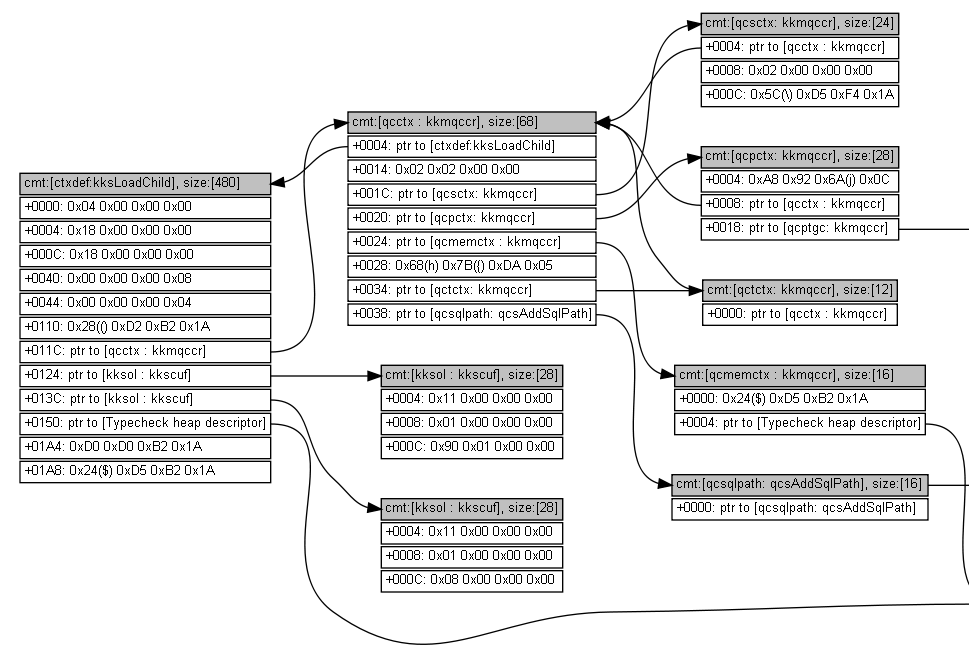
\includegraphics[scale=0.55]{advanced/450_more_ptrs/oracle2_crop.png}
\end{figure}

Images plus grosses:
\href{https://raw.githubusercontent.com/DennisYurichev/RE-for-beginners/master/advanced/450_more_ptrs/oracle1.png}{1},
\href{https://raw.githubusercontent.com/DennisYurichev/RE-for-beginners/master/advanced/450_more_ptrs/oracle2.png}{2}.

Ceci est assez impressionnant, compte tenu du fait que je n'ai aucune information
à propos des types de données de toutes ces structures.
Mais je peux en obtenir des informations.

\subsubsection{Maintenant le ramasse miette pour C/C++: Boehm GC}

\myindex{Garbage collector}
Si vous utilisez un bloc alloué en mémoire, son adresse doit être présente quelque
part, comme un pointeur dans une structure ou un tableau dans un autre bloc alloué,
ou dans une structure allouée globale, ou dans une variable locale sur la pile.
S'il n'y a plus de pointeur sur un bloc, vous pouvez l'appeler "orphelin", et il
est une cause des fuites de mémoire.

Et c'est ce qu'un \ac{GC} fait.
Il balaye tous les blocs (car il garde un \oe{}il sur tous les blocs alloués) à
la recherche de pointeurs.
Il est important de comprendre qu'il n'a aucune idée du type de données de tous les
champs de ces structures dans le blocs---ceci est important, le \ac{GC} n'a aucune information
sur les types.
Il balayage juste les blocs à la recherche de mots 32-bit ou 64-bit, et regarde s'ils
peuvent être des pointeurs sur d'autres bloc(s).
Il balaye aussi la pile.
Il traite les blocs alloués et la pile comme des tableaux de mots, dont certains pourraient
être des pointeurs.
Et s'il trouve un bloc alloué, qui est "orphelin", i.e., sur lequel aucun autre pointeur
sur lui depuis un autre bloc ou la pile, ce bloc est considéré comme inutile, devant
être libéré.
Le processus de balayage prend du temps, et c'est pourquoi les \ac{GC}s sont critiqués.

\myindex{Boehm garbage collector}
Ainsi, un \ac{GC} comme celui de Boehm\footnote{\url{https://www.hboehm.info/gc/}}
(pour du C pur) possède une fonction comme \verb|GC_malloc_atomic()|---en l'utilisant,
vous  déclarez que le bloc alloué avec cette fonction ne contiendra jamais de pointeur
vers un autre bloc.
Ça peut être une chaîne de texte, ou un autre type de donnée.
(En effet, \verb|GC_strdup()| appelle \verb|GC_malloc_atomic()|.)
Le \ac{GC} ne va pas le balayer.

% Even more: if \ac{GC}'s memory allocator thinks it can find a better place for a block, it can \emph{move} it to another place, and then fix (rewrite) all addresses,
% pointing to it, in all other blocks and in stack.


